% !TeX root = ../thuthesis-example.tex

\chapter{优化空间扩展}
\thusetup{
  cite-style = super,
}

\section{灵活规约定义}
规约是稀疏稠密混合张量代数的核心操作。规约的数学定义如式\eqref{eq:reduction}。其中$x \in X$,每个$x$有两个参数,一个是$id\in ID$,另一个是$val$。其中$id$是可以哈希的键值,$val$是可以被运算符$\oplus$运算的值。
$X$是由$x$组成的列表,$Out$是输出列表,由$ID$索引。

\begin{equation}
  Out[i] = \oplus_{x\in X;x.id=i} x.val
  \label{eq:reduction}
\end{equation}
\begin{figure}[h]%
  \centering
  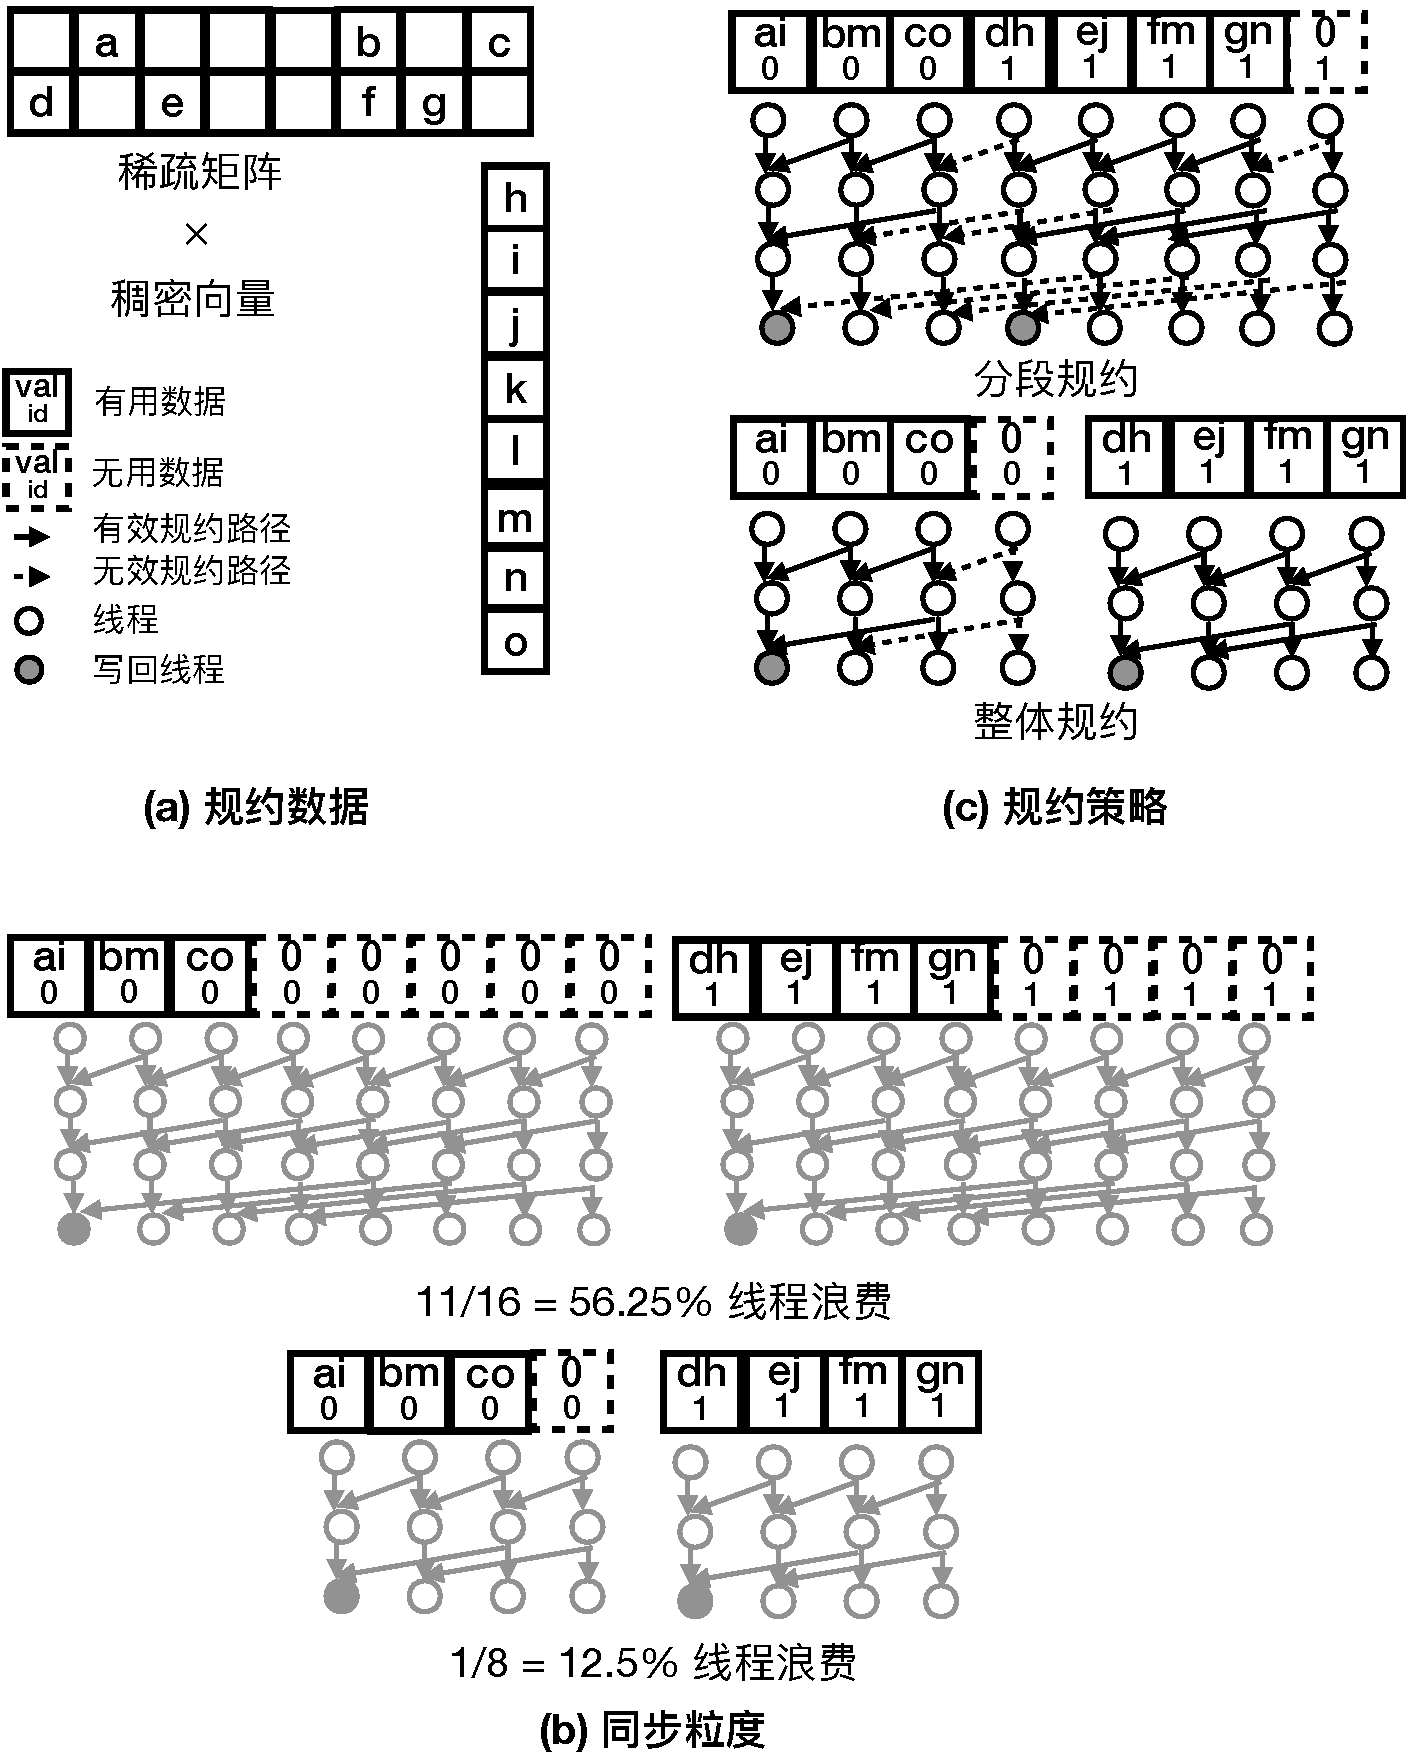
\includegraphics[width=0.5\textwidth]{reduction.pdf}
  \caption{不同规约粒度和规约方法。(a)图示和供规约的例子。其中有一个行数为2列数为8的稀疏矩阵和一个长度为8的稠密向量做矩阵向量乘法。(b)不合适的规约粒度会导致线程浪费,该子图中未区分有效和无效规约路径。(c)分段规约和整体规约。在这个例子中分段规约有2个写回线程。整体规约始终只有1个写回线程。}
  \label{fig:reductions}
\end{figure}
同时,不同的规约粒度也可能影响线程利用率,进一步影响算子性能。PRedS\cite{yu2021exploiting}虽然研究了并行规约粒度对性能的影响,但是它只局限于$X$中所有元素的$id$相等的情况,即稠密规约。本文更进一步,研究稀疏规约,即$X$中元素的$id$不相等的情况。
因为$id$不相等,所以不是所有元素都要累加到同一个输出上。因此,本文引入了有用数据,无用数据,有效规约路径,无效规约路径,和写回线程等概念。
这些概念的产生与GPU的线程同步策略密切相关。GPU会同步一组线程,而这组线程的线程数是2的次方且不大于32。这组线程的线程数我们称之为同步粒度。线程可以向同一线程组的另一的线程种传递本线程持有的寄存器数据。有用数据的意思是对最后结果起作用的数据,即$X$中的元素。无用数据是规约粒度和待规约元素个数不匹配引入的数据。在图\ref{fig:reductions}(b)的两个例子中,均采用整体规约。
因为整体规约要求所有被规约元素的$id$相同,所以当规约粒度超过$id$相同的元素数目时,就需要补充一些$val$是$\oplus$运算意义下的零元(在实数加法中就是0)的元素。这些元素只是起到占位作用,其$val$并没有加到输出结果中,因此被称为无用数据。
相应地,有效规约路径表示该路径连接的两种线程中,起始线程的值会最终叠加到写回线程的值中。无效规约路径则是为了避免GPU各线程执行路径不一致问题而引入的执行路径。
GPU提供了多种规约方式,写回线程表示该线程的寄存器中存放着最终写入$Out$的数据。分段规约表示一个线程组规约给定数目的$X$中的元素,整体规约表示一个线程组规约$X$中给定$id$的元素。分段规约根据该线程组处理的不同$id$数量可以有多个写回线程,整体规约因此$id$相同,所以只有1个写回线程。多个写回线程的线程号取决于$X$中的$id$分布,因此在运行时决定。两种规约的示意图如图\ref{fig:reductions}(c)所示。
不同的输入数据适合不同的规约,比如在\cite{dai2022heuristic}的对比实验中,分段规约和整体规约在不同数据集上的性能既可能好,也可能差2到4倍。

\section{灵活规约优化空间扩展}
\subsection{硬件模型}
因为规约是稀疏稠密混合张量代数的核心操作,所以优化空间扩展核心是多少数据需要被规约以及采用何种规约策略。本文将逻辑上原子的计算单元设置为线程。一个线程可以一个串行程序。所有线程独立执行相同的程序。每个线程有各自的输入数据,同时根据threadId区分。
线程可以成组做同步规约,规约并行度(粒度)可以是2,4,8,16或32.我们将GPU的计算建模为逻辑上无限多的平行线程,同时定义GPU可以提供的线程数为源并行度。在这个模型中我们没有考虑共享内存、线程块层级以及线程到流式处理器的映射策略等。本文把这些视作在基础并行模式确定后合理的部署细节。换句话说,在本文基于灵活规约扩展后的优化空间中,每一种优化策略对应许多不同的部署技术。这样扩展后的优化空间可以为GPU细节优化提供更简洁的视角。
\subsection{原子并行}
为了具体定义并行模式,本文提出了原子并行概念。处于原子并行状态的一个程序不能继续被并行。换句话说,原子并行规定了一个线程执行的数据量。正式地,本文定义原子并行是最小数据的笛卡尔积。最小数据数据是一个线程所能处理的最小某类数据量。原子并行可以用来构建在GPU上执行的稀疏稠密混合代数的优化空间。
当然分块技术、精细管理共享内存、线程映射等优化技术对于GPU上的稀疏稠密混合代数也很重要\cite{hidayetouglu2020scale,mehrabi2021learning,xin2021fast,gale2020sparse}。这些技术对于稠密张量相对稀疏张量形状较大时更有利,比如在SpMM中稠密矩阵列数大于128时。因为计算的负载会很重,想稠密矩阵的向量化数据读取会成为瓶颈。
当稠密张量相对于稀疏张量形状较小,比如SpMM中稠密矩阵列数小于8时,每个线程的工作负载都较小,此时执行时间被最长的线程组执行时钟数限制,因此需要更好的工作负载均衡。

下面以SpMM为例展示利用原子并行构建灵活规约优化空间扩展的步骤。SpMM有两种正交的原子并行:最小数据可以是$\{\frac{1}{g},1,g\}$个稀疏矩阵的非零元和$\{\frac{1}{c},1,c\}$个稠密矩阵列;也可以是$\{\frac{1}{g},1,g\}$个稀疏矩阵行和$\{\frac{1}{c},1,c\}$个稠密矩阵列。
其中$c\in \mathbb{Z^+}$和$g\in \mathbb{Z^+}$是可以调优的参数。尽管他们都可以是1但是他们和1的意义不同,因为他们是可以调优的。因此基于原子并行的SpMM灵活规约粒度优化空阿金扩展可以用$<x\,nnz , y\,col>$或者$<x\,row, y\,col>$描述。
源并行度只会向原子并行度中的一个元素做乘法。例如,给定源并行度$r$,针对第一种原子并行线程执行的数据量可以定义为$<r \times x\,nnz , y\,col>$或者$<x\,nnz, r \times y\,col>$;针对第二种原子并行线程执行的数据量可以定义为$<r \times x\,row , y\,col>$或者$<x\,row, r \times y\,col>$。
除此以外,分数类型的数据意味着不同线程会在同样的单个数据上执行。比如$<\frac{1}{g}\, row, 1\, col>$表示$g$个线程合作在同一行上执行。
\subsection{空间定义}
依然使用SpMM的例子,我们用原子并行和规约并行 $\{<...>,r\}$ 来定义一个SpMM算子。$<...>\in \{\frac{1}{g},1,g\}\, nnz \times \{\frac{1}{c},1,c\}\, col $ or $\{\frac{1}{g},1,g\}\,row \times \{\frac{1}{c},1,c\}\,col$。他们描述了最小数据。同时规约并行度$r\in\{2,4,8,16,32\}$指定了每次有多少线程同步。 
图\ref{fig:space3d}展示了SpMM的优化空间。但是,基于原子并行和规约并行构建的优化空间中不是所有点都合法。图\ref{fig:space}中展示了空间剪枝的细节。优化空间中合法的点有3个条件
\begin{enumerate}
  \item $\{<\frac{1}{g}\,nnz , x\,col>,r\}$, $\{<x\,nnz , \frac{1}{c}\,col>,r\}$ 
  是合法的,因为一个非零元一定与稠密矩阵中的一个点相乘。
  \item $\{<\frac{1}{g}\,row, x\,col>,r\}(\frac{r}{g}<1)$
  是非法的,因为整体规约只能有一个写回线程。
  \item $\{<\frac{1}{g}\,row , \frac{1}{c}\,col>,r\}$
  是非法的,因为它和源并行只能与原子并行中的一个元素相乘矛盾
\end{enumerate}
\begin{figure}[h]%
  \centering
  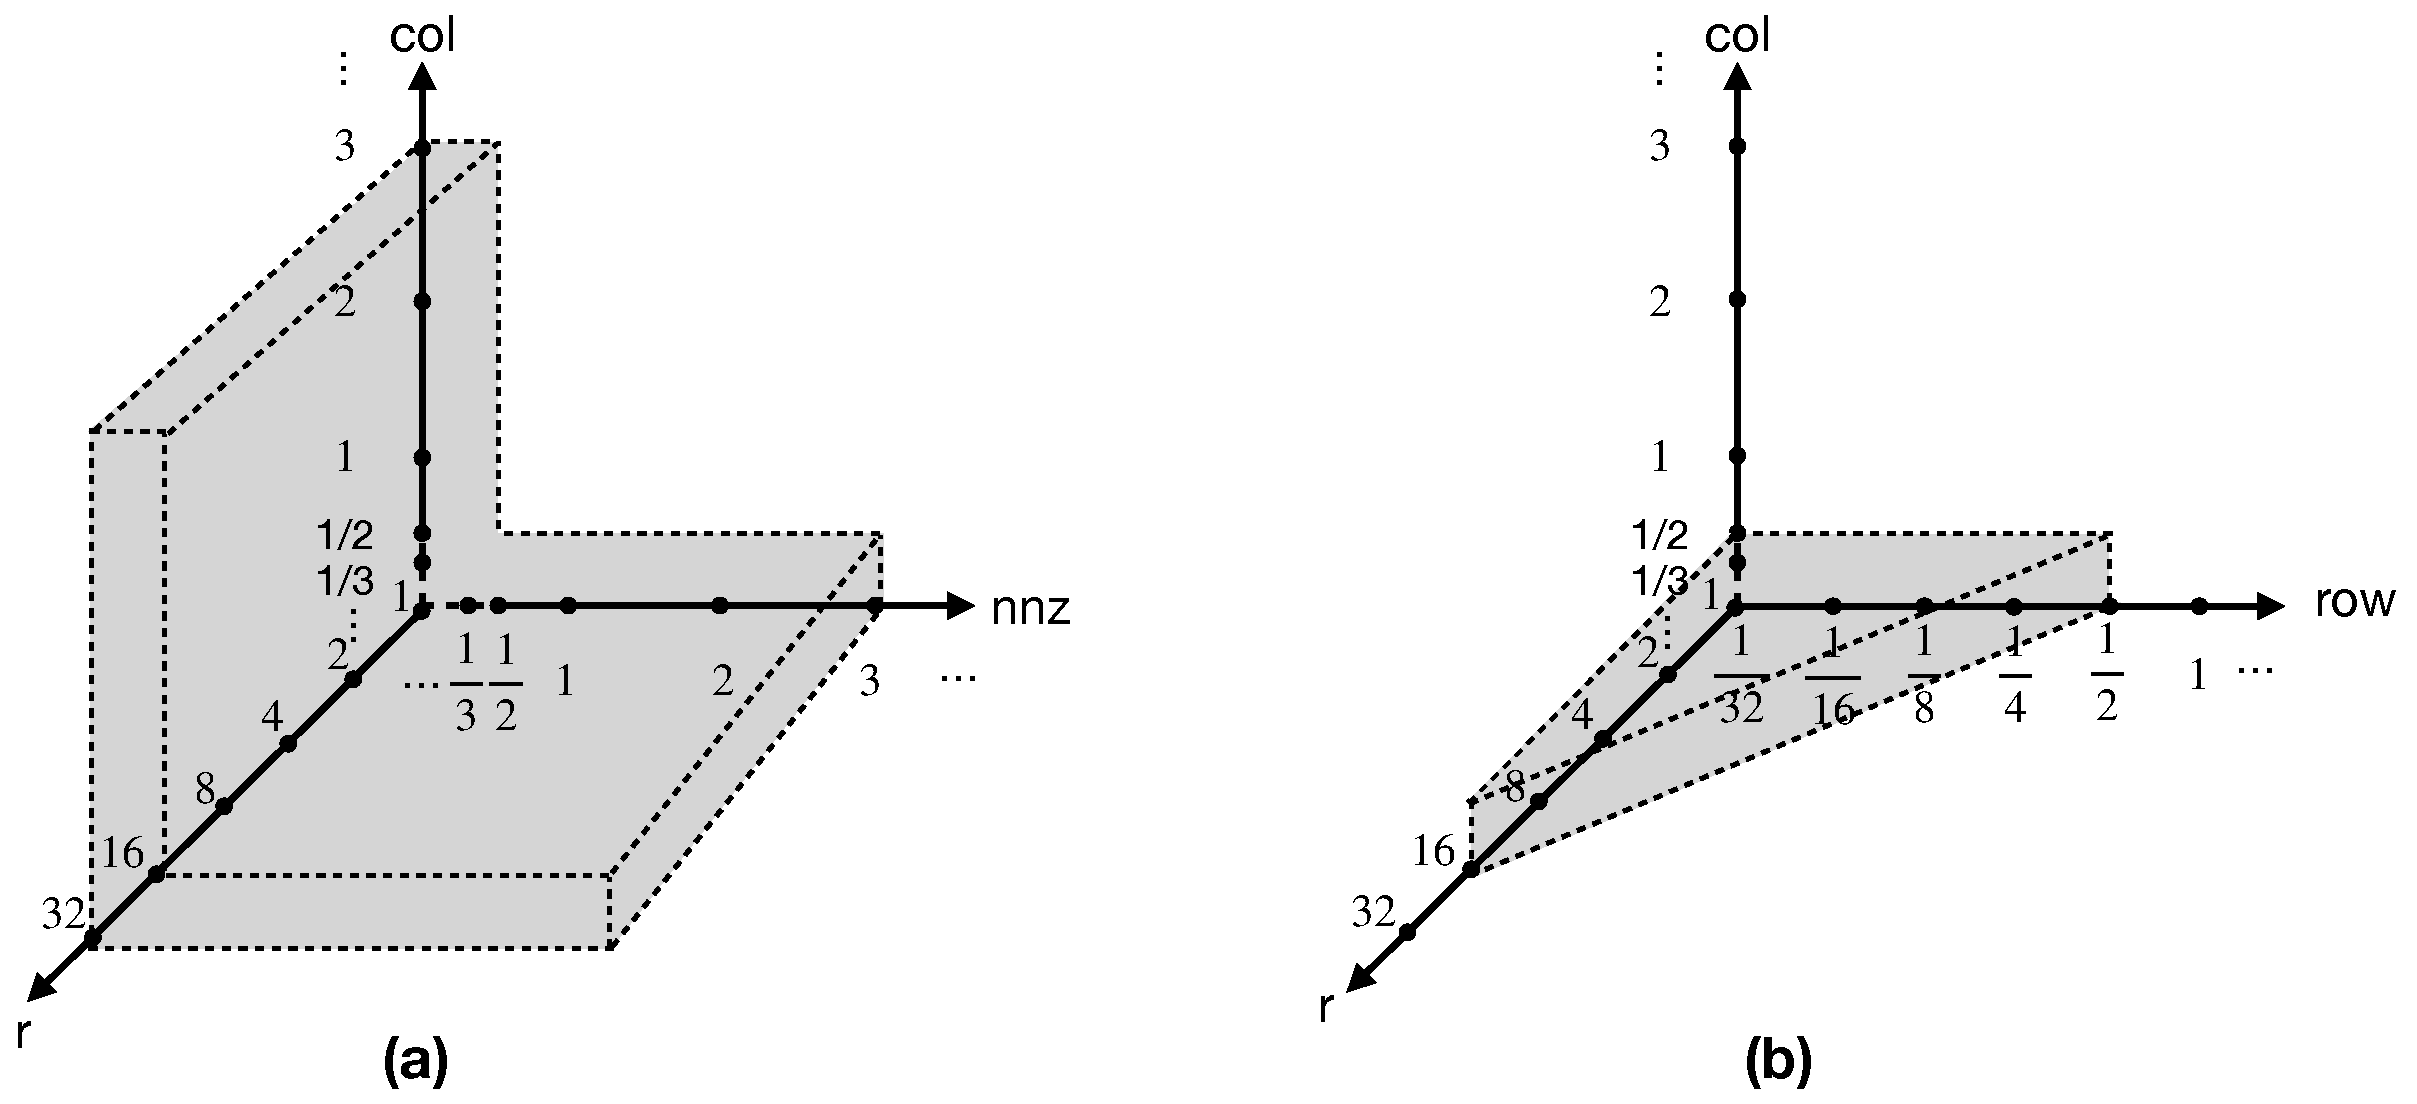
\includegraphics[width=0.9\textwidth]{space_3d.pdf}
  \caption{SpMM的灵活规约优化空间扩展,灰色区域是非法区域,在每个坐标轴根部的虚线部分代表结束点和硬件相关。}
  \label{fig:space3d}
\end{figure}
\begin{figure}[h]%
  \centering
  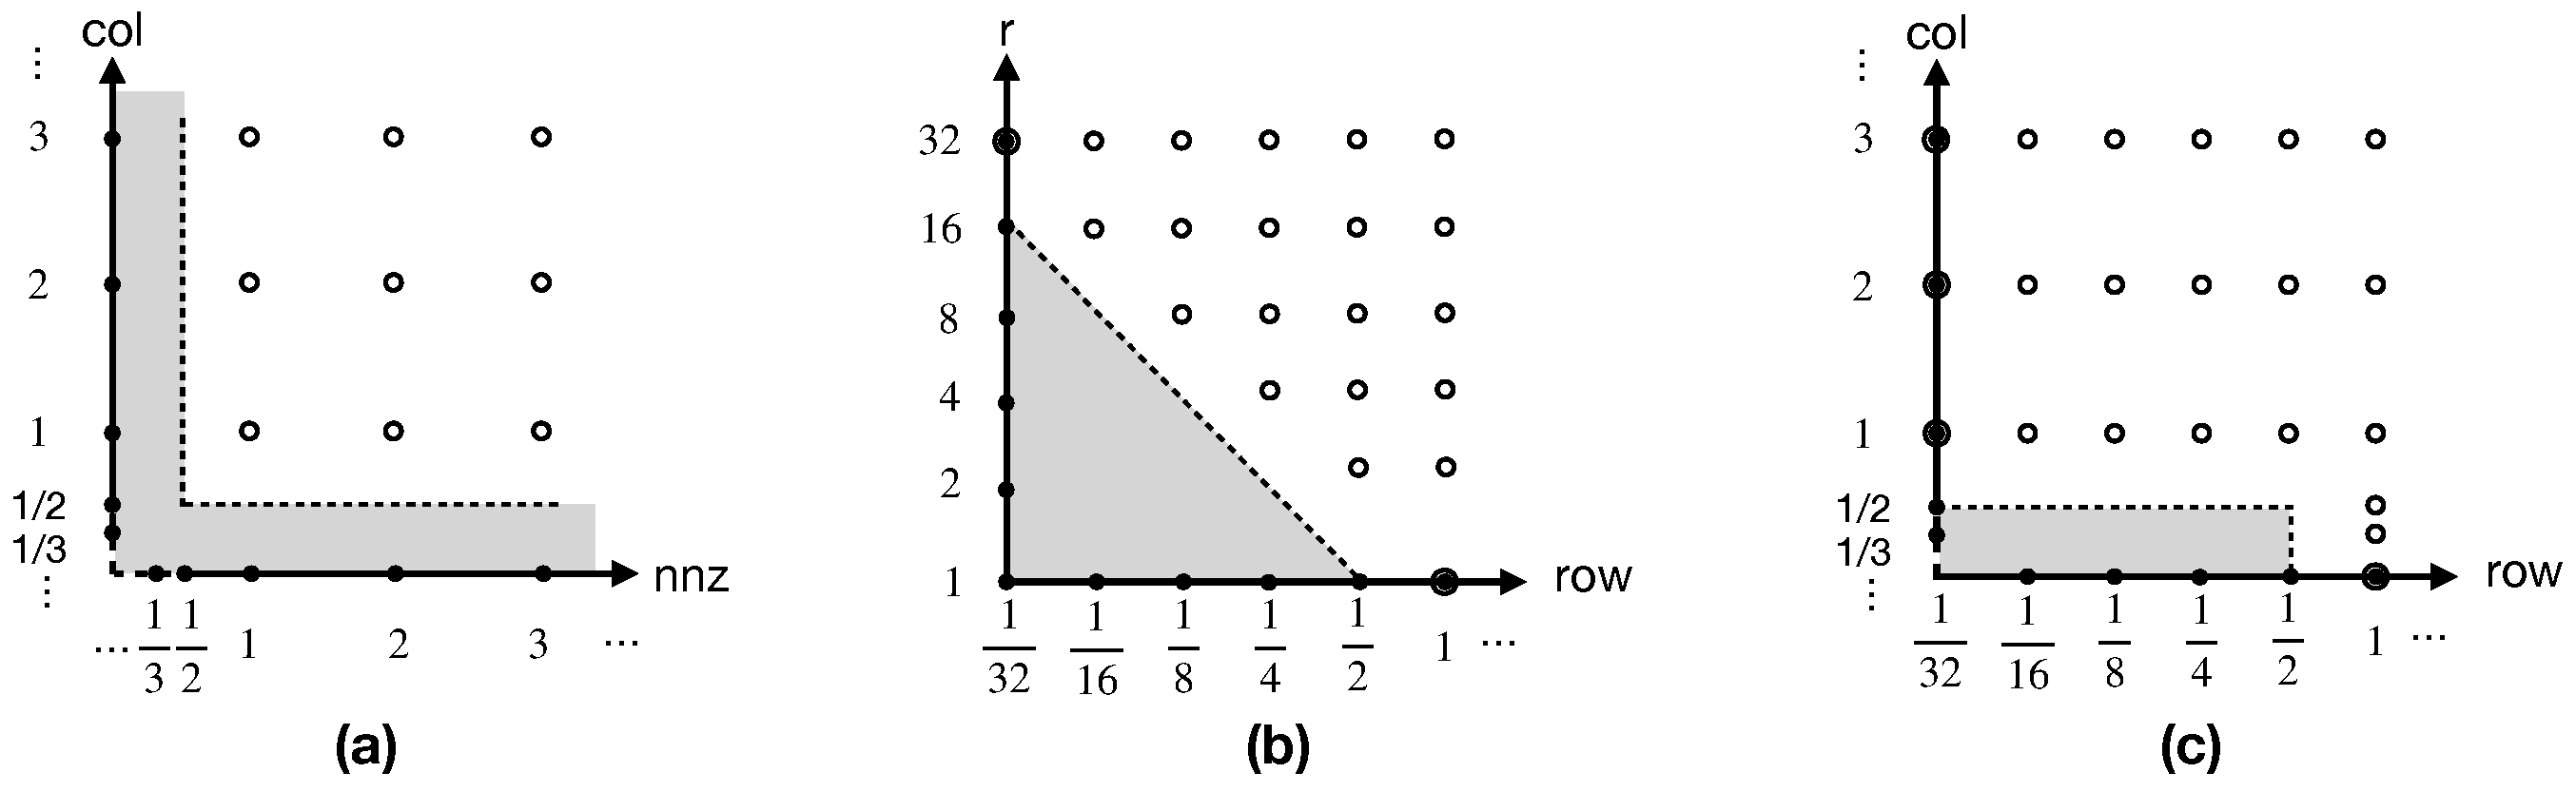
\includegraphics[width=0.9\textwidth]{space.pdf}
  \caption{SpMM优化空间的投影。灰色区域是非法的,空心圈是合法的点。子图(a),(b),(c)分别对应规则1,2,,3。}
  \label{fig:space}
\end{figure}
最新的SpMM算子库设计空间DA-SpMM包含在上面基于原子并行构建的灵活规约优化空间扩展中。DA-SpMM提出了一个三维的SpMM算法设计空间,分别有三个维度:行/非零元均衡、行/列起始循环,并行/串行规约,论文中分别简称RB/EB、RM/CM、PR/SR。
因为行/列起始循环不影响并行策略,所以我们只考虑EB+PR,RB+PR,EB+SR,RB+SR四种算法。如图\ref{fig:daspmm}所示,在灵活规约优化空间扩展中EB+PR是$\{<1\,nnz , c\,col>,32\}$,RB+PR是$\{<\frac{1}{32}\,row, c\,col>,32\}$,EB+SR是$\{<32\,nnz,c\,col >,1\}$,
RB+SR是$\{<1\,row,c\,col >,1\}$。其中$c$对应DA-SpMM中的向量化参数,$g$表示灵活规约中的线程组大小。尽管在真实GPU中由于源并行度有限,导致$1\,row$或$1\,nnz$可能会有超过1行或1个非零元的最小数据。但是我们仍然将这类算法归类为空间中的$1\,row$或$1\,nnz$点。
\begin{figure}[h]%
  \centering
  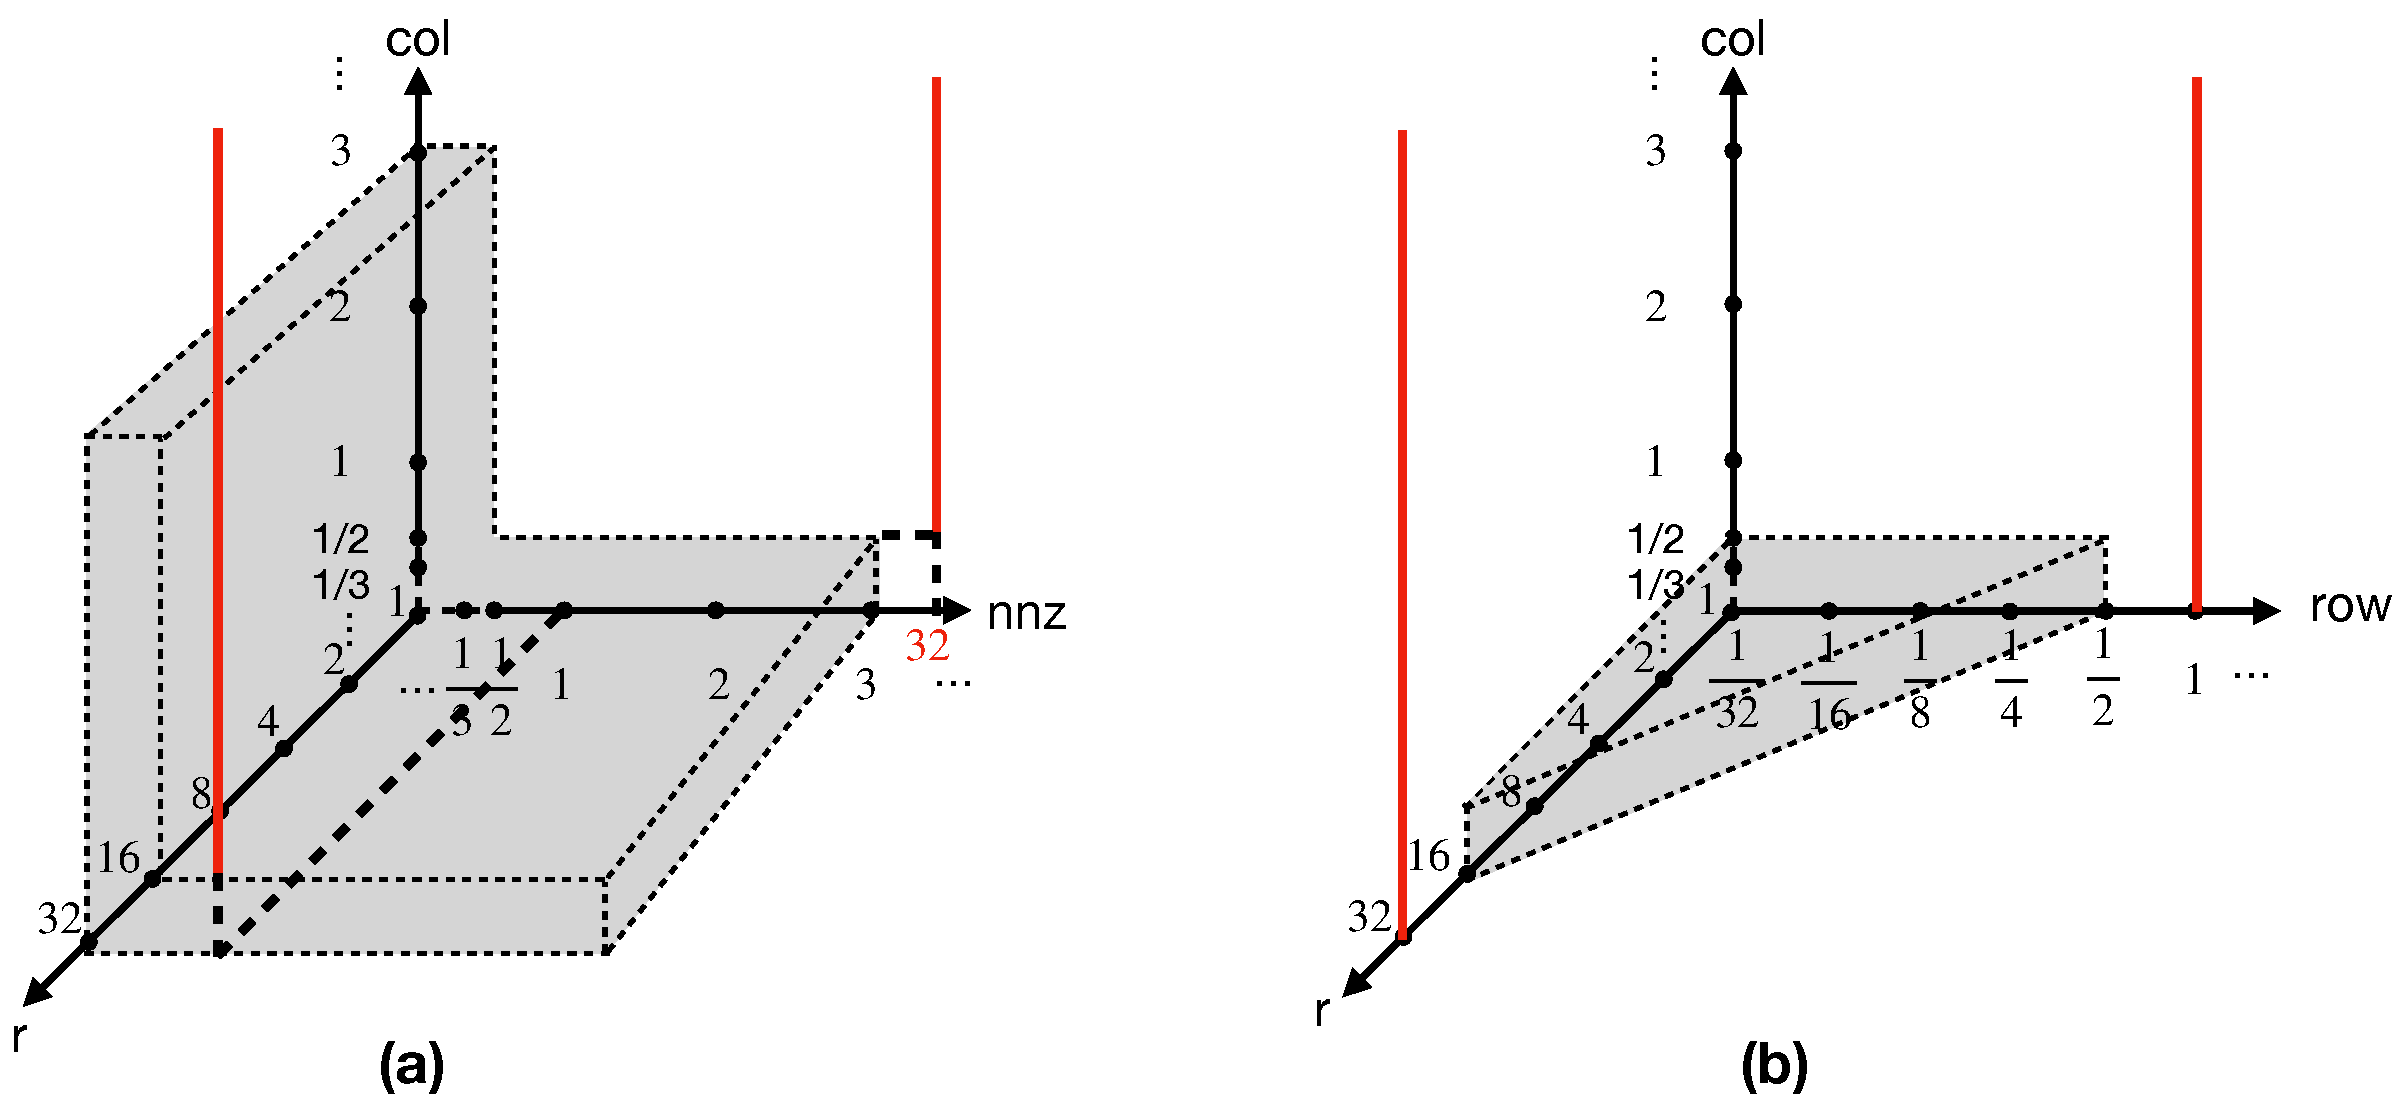
\includegraphics[width=0.9\textwidth]{daspmm.pdf}
  \caption{DA-SpMM的四种算法在灵活规约优化空间扩展中的位置,红色代表DA-SpMM包含的优化空间,灰色区域是非法区域,在每个坐标轴根部的虚线部分代表结束点和硬件相关。}
  \label{fig:daspmm}
\end{figure}

\section{实验结果}
